\section{Adatbázisséma}

\subsection{Tervezés}

Az adatbázisséma tervezéséhez a dbdiagram.io nevű platformfüggetlen, webes ER diagram tervező szoftvert használtam.
Ez egy saját fejlesztésű, DBML nevű DSL nyelvet használ a séma leírására, és lehetővé teszi ennek exportálását különféle formátumokba.

\begin{figure}[!ht]
\centering
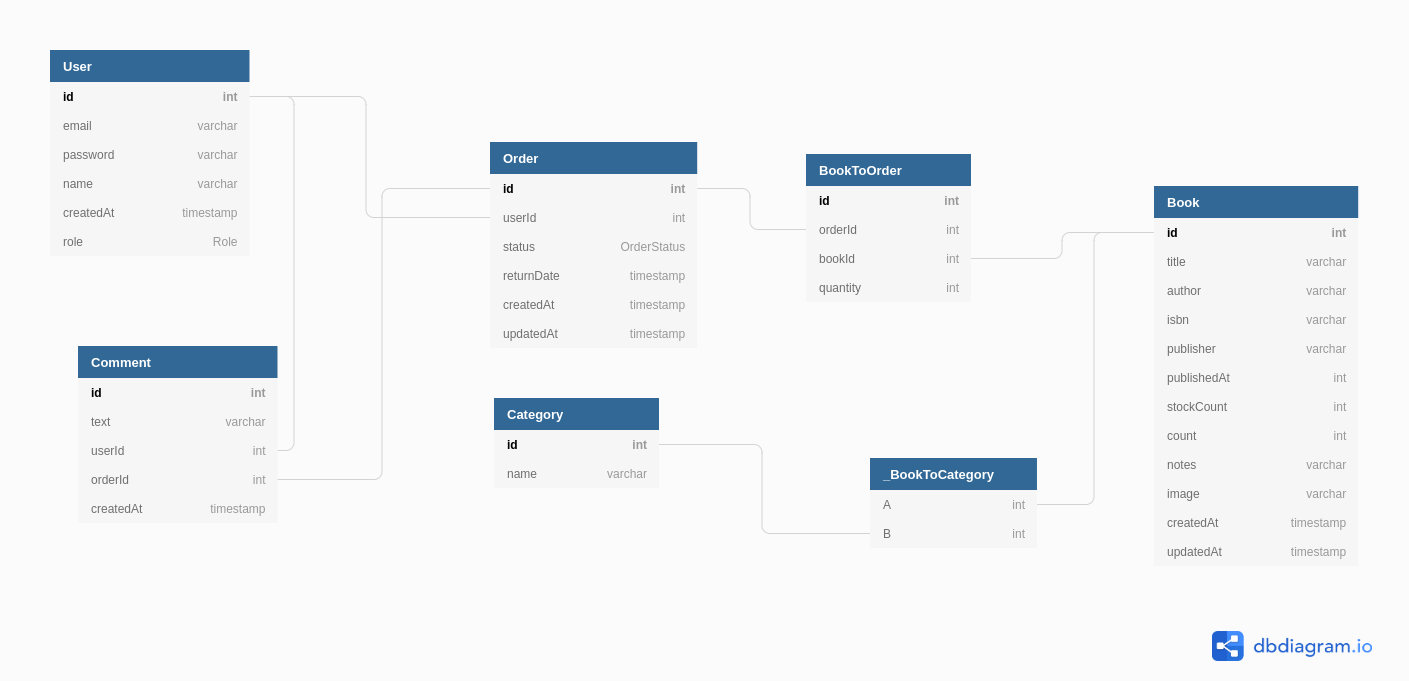
\includegraphics[width=150mm, keepaspectratio]{figures/dbschema.png}
\caption{Az adatbázisséma ER diagramja.}
\label{fig:DBSchema}
\end{figure}

A séma tervezése során a Prisma által használt elnevezési konvenciókat használtam, hogy megkönnyítsem a két technológia közötti átjárhatóságot.

\subsection{Implementáció}

A séma adatbázisba történő átvezetésére két lehetőségünk van. Az egyik, hogy a dbdiagram oldalról lehetőségünk van .sql kiterjesztésű fájlt letölteni,
ezt a létrehozott adatbázisunkon futtatni, majd a Prisma introspect funkcióját használva legenerálni hozzá a Prisma schema fájlt a backendünk számára.
A másik, egyszerűbb megoldás a Prisma migrate használata. Ez esetben nekünk manuálisan kell létrehozni a Prisma schema fájlt a
korábbi diagram alapján, majd a
\begin{lstlisting}
prisma migrate save --experimental
prisma migrate up --experimental
\end{lstlisting}

parancsokat kiadva létrehozzuk és futtatjuk a Prisma migrációt.
Ez utóbbi módszer előnye, hogy kevesebb lépéssel tölthető be az adatbázisba a kívánt séma, valamint képes a séma felépítését és
változását adatbázisfüggetlen módon követni.

Bár a Prisma ezen funkciója egyelőre csak experimental státuszban van,
a program fejlesztése közben a működésében nem tapasztaltam fennakadást, így ezen módszer alkalmazása mellett döntöttem.
